\documentclass[border=8pt]{standalone}
\usepackage{amsmath,amssymb,bm}
\usepackage{xcolor}
\usepackage{tikz}
\definecolor{P}{HTML}{4B1D8F}
\definecolor{ink}{HTML}{1B1B2F}
\definecolor{X}{HTML}{C2386B}
\colorlet{rule}{P!45!white}
\begin{document}
\Large
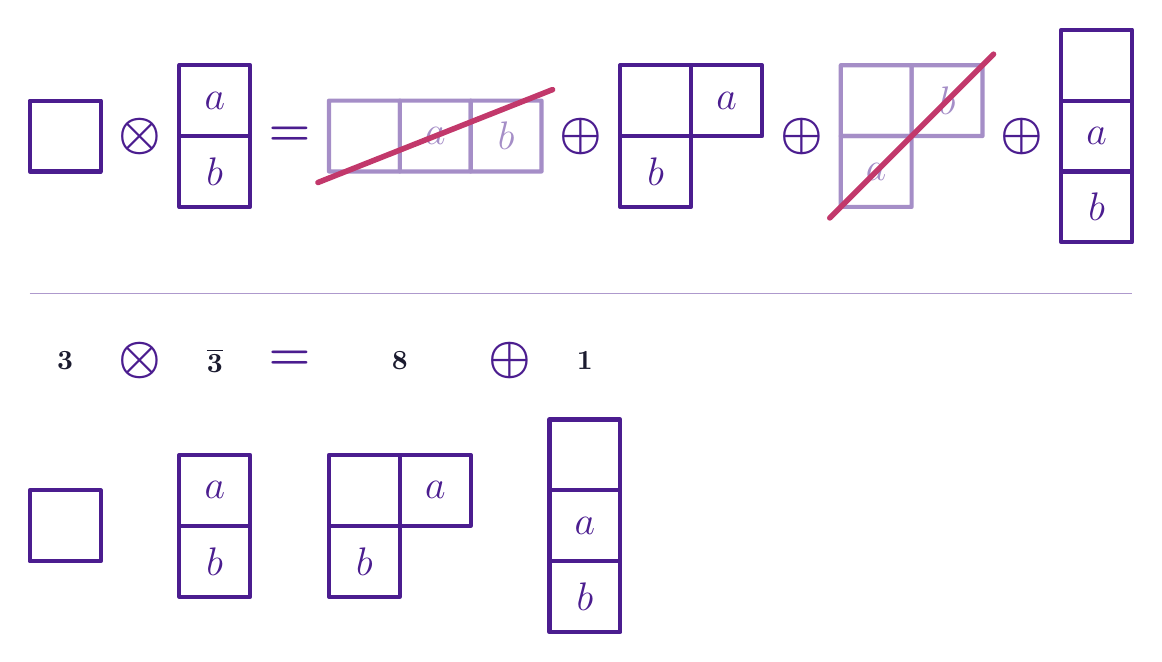
\begin{tikzpicture}[every node/.style={text=ink}]
\draw[P,line width=1.5pt,line join=round] (0.000,0.450) rectangle (0.900,-0.450);
\node[text=P] at (1.400,0.000) {\LARGE$\bm{\otimes}$};
\draw[P,line width=1.5pt,line join=round] (1.900,0.900) rectangle (2.800,0.000);
\node[text=P] at (2.350,0.450) {\Large$a$};
\draw[P,line width=1.5pt,line join=round] (1.900,0.000) rectangle (2.800,-0.900);
\node[text=P] at (2.350,-0.450) {\Large$b$};
\node[text=P] at (3.300,0.000) {\LARGE$\bm{=}$};
\begin{scope}[transparency group,opacity=.5]
\draw[P,line width=1.5pt,line join=round] (3.800,0.450) rectangle (4.700,-0.450);
\draw[P,line width=1.5pt,line join=round] (4.700,0.450) rectangle (5.600,-0.450);
\node[text=P] at (5.150,0.000) {\Large$a$};
\draw[P,line width=1.5pt,line join=round] (5.600,0.450) rectangle (6.500,-0.450);
\node[text=P] at (6.050,0.000) {\Large$b$};
\end{scope}
\draw[X,line width=2pt,line cap=round] (3.660,-0.590) -- (6.640,0.590);
\node[text=P] at (7.000,0.000) {\LARGE$\bm{\oplus}$};
\draw[P,line width=1.5pt,line join=round] (7.500,0.900) rectangle (8.400,0.000);
\draw[P,line width=1.5pt,line join=round] (8.400,0.900) rectangle (9.300,0.000);
\node[text=P] at (8.850,0.450) {\Large$a$};
\draw[P,line width=1.5pt,line join=round] (7.500,0.000) rectangle (8.400,-0.900);
\node[text=P] at (7.950,-0.450) {\Large$b$};
\node[text=P] at (9.800,0.000) {\LARGE$\bm{\oplus}$};
\begin{scope}[transparency group,opacity=.5]
\draw[P,line width=1.5pt,line join=round] (10.300,0.900) rectangle (11.200,0.000);
\draw[P,line width=1.5pt,line join=round] (10.300,0.000) rectangle (11.200,-0.900);
\node[text=P] at (10.750,-0.450) {\Large$a$};
\draw[P,line width=1.5pt,line join=round] (11.200,0.900) rectangle (12.100,0.000);
\node[text=P] at (11.650,0.450) {\Large$b$};
\end{scope}
\draw[X,line width=2pt,line cap=round] (10.160,-1.040) -- (12.240,1.040);
\node[text=P] at (12.600,0.000) {\LARGE$\bm{\oplus}$};
\draw[P,line width=1.5pt,line join=round] (13.100,1.350) rectangle (14.000,0.450);
\draw[P,line width=1.5pt,line join=round] (13.100,0.450) rectangle (14.000,-0.450);
\node[text=P] at (13.550,0.000) {\Large$a$};
\draw[P,line width=1.5pt,line join=round] (13.100,-0.450) rectangle (14.000,-1.350);
\node[text=P] at (13.550,-0.900) {\Large$b$};
\draw[rule,line width=.7pt] (0,-2.0) -- (14.000,-2.0);
\node at (0.450,-2.850) {$\mathbf{3}$};
\draw[P,line width=1.5pt,line join=round] (0.000,-4.500) rectangle (0.900,-5.400);
\node[text=P] at (1.400,-2.850) {\LARGE$\bm{\otimes}$};
\node at (2.350,-2.850) {$\overline{\mathbf{3}}$};
\draw[P,line width=1.5pt,line join=round] (1.900,-4.050) rectangle (2.800,-4.950);
\node[text=P] at (2.350,-4.500) {\Large$a$};
\draw[P,line width=1.5pt,line join=round] (1.900,-4.950) rectangle (2.800,-5.850);
\node[text=P] at (2.350,-5.400) {\Large$b$};
\node[text=P] at (3.300,-2.850) {\LARGE$\bm{=}$};
\node at (4.700,-2.850) {$\mathbf{8}$};
\draw[P,line width=1.5pt,line join=round] (3.800,-4.050) rectangle (4.700,-4.950);
\draw[P,line width=1.5pt,line join=round] (4.700,-4.050) rectangle (5.600,-4.950);
\node[text=P] at (5.150,-4.500) {\Large$a$};
\draw[P,line width=1.5pt,line join=round] (3.800,-4.950) rectangle (4.700,-5.850);
\node[text=P] at (4.250,-5.400) {\Large$b$};
\node[text=P] at (6.100,-2.850) {\LARGE$\bm{\oplus}$};
\node at (7.050,-2.850) {$\mathbf{1}$};
\draw[P,line width=1.5pt,line join=round] (6.600,-3.600) rectangle (7.500,-4.500);
\draw[P,line width=1.5pt,line join=round] (6.600,-4.500) rectangle (7.500,-5.400);
\node[text=P] at (7.050,-4.950) {\Large$a$};
\draw[P,line width=1.5pt,line join=round] (6.600,-5.400) rectangle (7.500,-6.300);
\node[text=P] at (7.050,-5.850) {\Large$b$};
\end{tikzpicture}
\end{document}
